
%\begin{figure}
%\includegraphics[width=\textwidth]{titel-stadtzentrum-desktop.png}
%\end{figure}
\begin{titlepage}
\vspace*{3cm}
\begin{center}
    
\includegraphics[height=5cm]{../data/figures/milet-logo-tr}\\
    \vspace*{1cm}

    {\LARGE \textsc{\textbf{The Miletus Bibliography}}}\\

    \today\\
    \vspace*{2cm}

    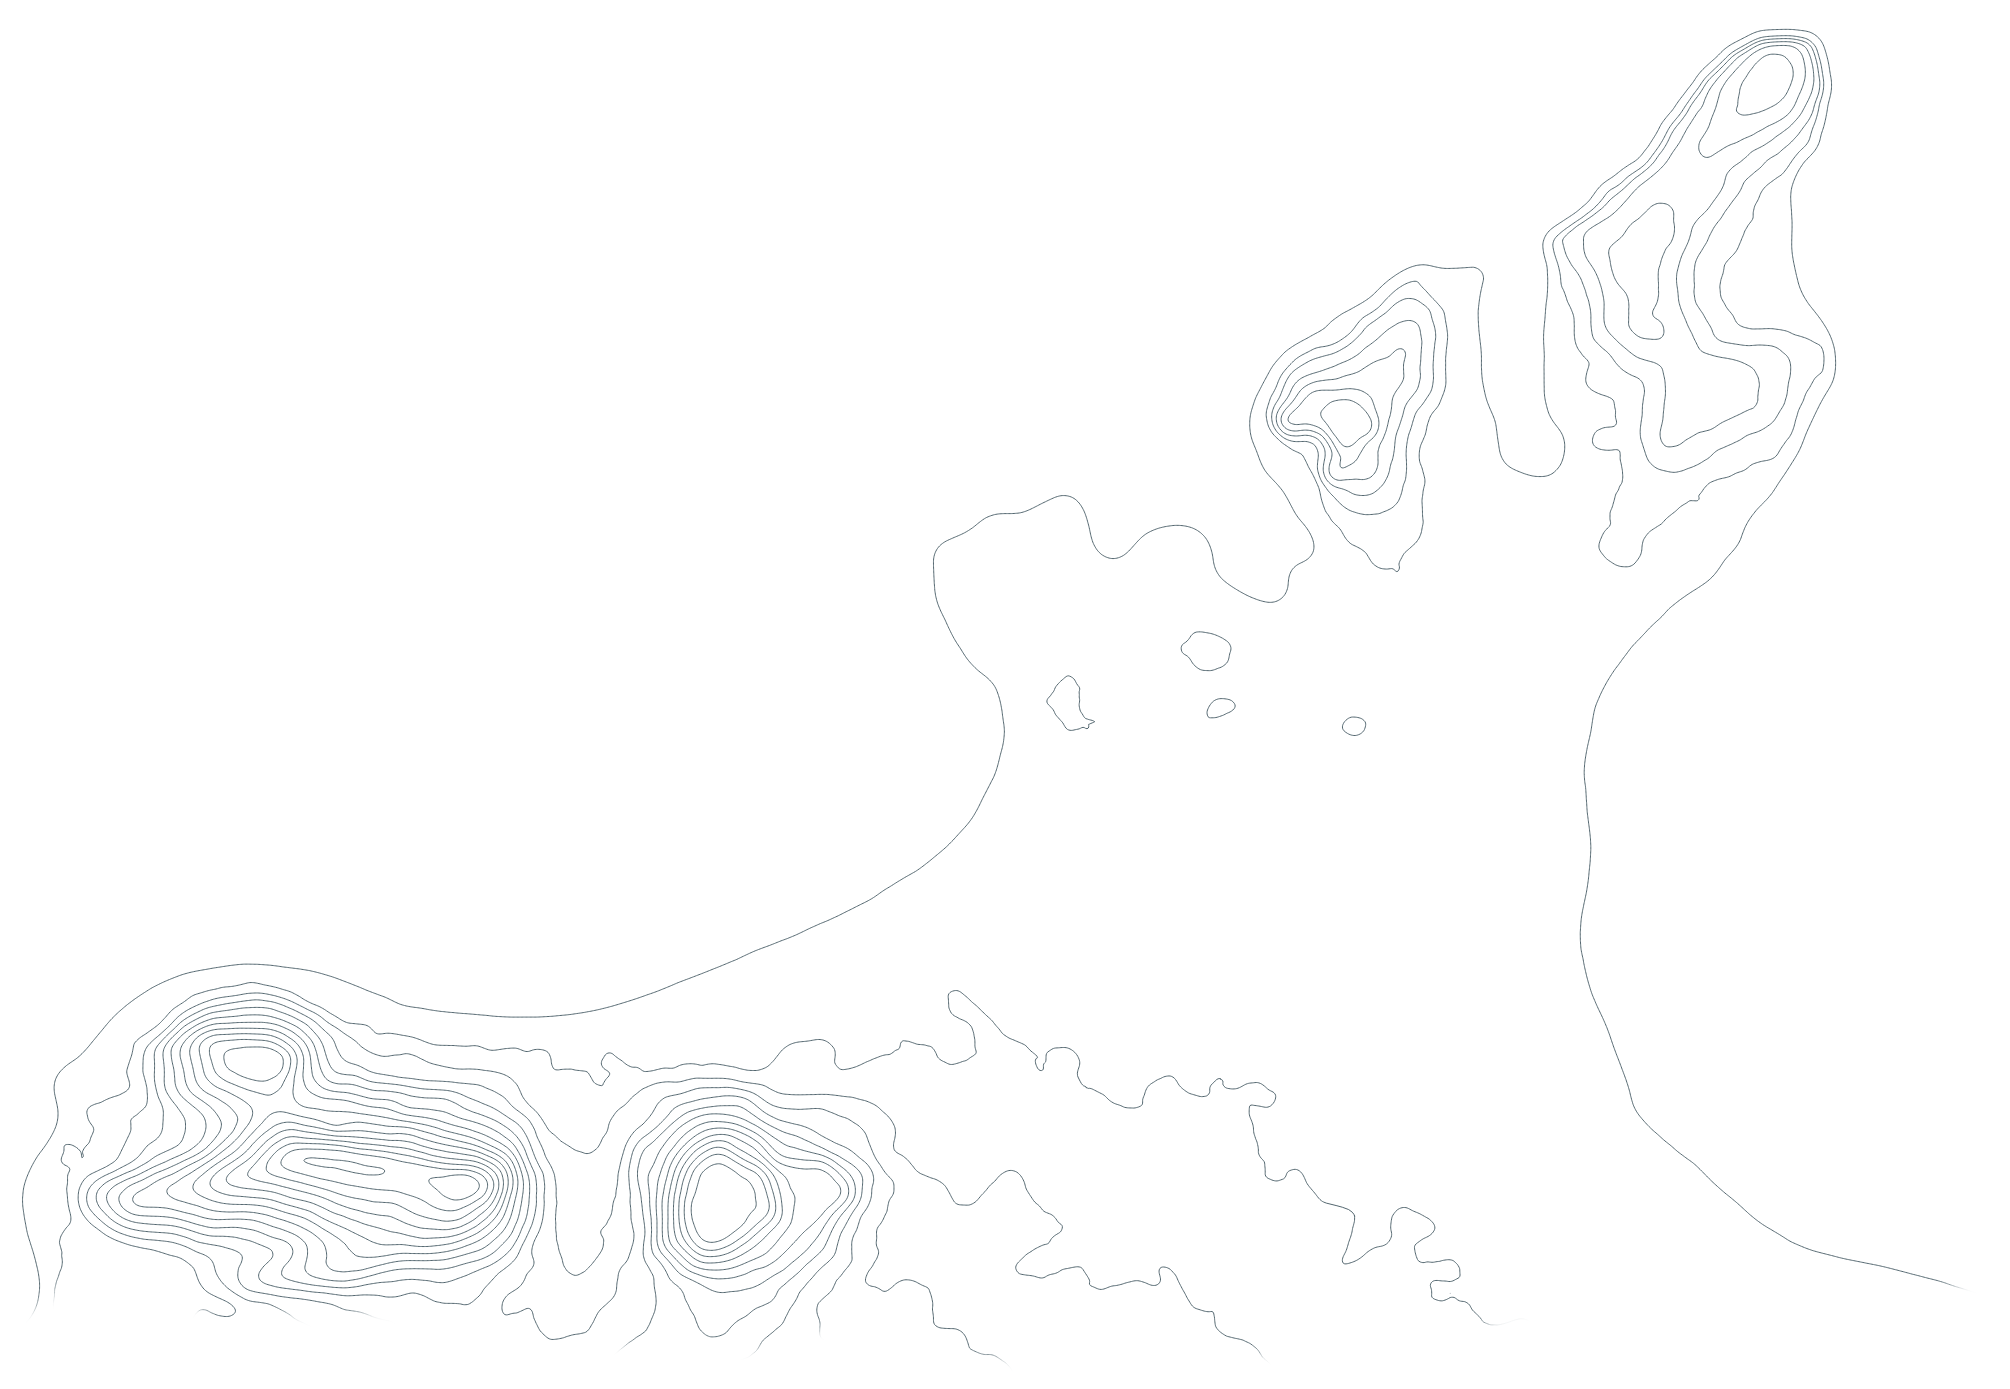
\includegraphics[width=0.8\textwidth]{../data/figures/Gelaende2.png}
\end{center}

\end{titlepage}

\chapter{Vorwort / Preface}
\pagenumbering{Roman}
\nocite{*}
\setcounter{page}{2}


\begin{tabular}[H!]{p{0.49\textwidth} c p{0.49\textwidth}}

Die Milet-Bibliographie wurde von Sabine Huy im Rahmen ihrer Tätigkeit für das Miletarchiv begründet und bis 2022 in dieser Form als \redhref{https://doi.org/10.25592/uhhfdm.8678}{PDF-Version zum Download} angeboten. Unter Mitarbeit von Caitlin Bamford und Silas Munnecke wurde die Liste zum Jahr 2022 in eine Datenbankversion überführt und wird seitdem von Lisa Steinmann gepflegt.  

& & 

The Miletus Bibliography has been offered as a \redhref{https://doi.org/10.25592/uhhfdm.8678}{PDF version for download} for many years by Sabine Huy in the course of her work at the Miletus Archive. With the collaboration of Caitlin Bamford and Silas Munnecke, the list was converted into a database version as of 2022 and has since been maintained by Lisa Steinmann.\\

Die Bearbeitung und Verwaltung der Bibliographie erfolgt in einer \redhref{https://www.zotero.org/groups/4475959/milet_bibliography}{öffentlich zugänglichen Zotero-Gruppenbibliothek}. Dieses Dokument ist ein \redhref{https://github.com/lsteinmann/Miletus_Bibliography}{automatisierter Export} der Bibliographie, die in durchsuchbarer Form auch auf der \redhref{https://www.miletgrabung.uni-hamburg.de/material/bibliographie.html}{Homepage der Miletgrabung} zur Verfügung steht. Dort gibt es ebenfalls die Möglichkeit, die Bibliographie in diversen Formaten für den Import in Literaturverwaltungsprogramme herunterzuladen.

& & 

The bibliography is edited and managed in a \redhref{https://www.zotero.org/groups/4475959/milet_bibliography}{publicly accessible Zotero group library}. This document is an \redhref{https://github.com/lsteinmann/Miletus_Bibliography}{automatically generated export} of the bibliography, which is also available in searchable form on the \redhref{https://www.miletgrabung.uni-hamburg.de/material/bibliographie.html}{homepage of the Miletus Excavation}. There is also an option there to download the bibliography in various formats for import into literature management software.\\

\end{tabular}

\vfill
\begin{tabular}{m{0.13\textwidth} m{0.13\textwidth} m{0.4\textwidth}}

\includegraphics[height=0.12\textwidth]{../data/figures/Logo.png} & 

\includegraphics[height=0.12\textwidth]{../data/figures/milet-logo-tr} & 
\redhref{https://www.miletgrabung.uni-hamburg.de}{www.miletgrabung.uni-hamburg.de} 
\redhref{mailto:miletgrabung@uni-hamburg.de}{miletgrabung@uni-hamburg.de}\\
\end{tabular}
